%presentation
\documentclass{beamer}

%impressions
%\documentclass[handout]{beamer}
%\usepackage{pgfpages}
%\pgfpagesuselayout{2 on 1}[a4paper,border shrink=5mm]
%\setbeameroption{notes on second screen}
%\pgfpagelayout{2 on 1}[a4paper, border, shrink=5mm]
% vue sur http://wwwtaketorg/spip/articlephp3?id_article=30...
%\usepackage[T1]{fontenc}
\usepackage[frenchb]{babel}
\usepackage[utf8x]{inputenc} % Pour pouvoir taper les accents sans faire de combinaison
%\usepackage{arev}
%\usepackage{aeguill}
%mode code
\usepackage{listings}

%mode verbatim
\usepackage{moreverb}

%\usepackage[darktab]{beamerthemesidebar}
%\leftsidebar
%\usetheme{Hannover}
%\usetheme{Warsaw}
%\usetheme{PaloAlto}
\usetheme{JuanLesPins}
%\usetheme{Antibes}
%\usetheme{Shingara}
%\usetheme{Berlin}
%\usetheme{Oxygen}
\usepackage{thumbpdf}
\usepackage{wasysym}
\usepackage{ucs}
\usepackage{pgfarrows,pgfnodes,pgfautomata,pgfheaps,pgfshade}
\usepackage{verbatim}
\usepackage{color}
\definecolor{links}{HTML}{2A1B81}
\hypersetup{colorlinks,linkcolor=,urlcolor=links}

\AtBeginSection[]
{
  \begin{frame}<beamer>
    \tableofcontents[currentsection,currentsubsection]
  \end{frame}
}

\usepackage[absolute,overlay]{textpos}
\newcommand{\source}[1]{\begin{textblock*}{10cm}(0cm,8.6cm)
    \begin{beamercolorbox}[ht=0.5cm,right]{framesource}
      \tiny
      \usebeamerfont{framesource}\usebeamercolor[fg]{framesource} Source: {#1}
    \end{beamercolorbox}
\end{textblock*}}

\title{Errbit}
\subtitle{pour dire c'est fix, \\ quand on vous remonte le bug}
\author{Cyril Mougel}
%\institute{AF83}
\date{4 Juillet 2013}

\logo{
\includegraphics[height=10mm]{errbit-logo.png}}

% Define you show the ruby code
\lstset{breaklines=true
    , language=ruby
    , numbers=left
    , tabsize=2
    , basicstyle=\small\ttfamily
    , keywordstyle=\color{blue}
    , commentstyle=\color{green}
    , stringstyle=\color{red}
    , identifierstyle=\ttfamily
    , columns=fixed
    , showstringspaces=false
}

\begin{document}

\begin{frame}
    \titlepage
\end{frame}

\begin{frame}
  \center{}
  \Huge{}
  Vous codez sans Bug?
\end{frame}

\begin{frame}
  \center{}
  \Huge{}
  Vous faites des tests Unitaires?
\end{frame}

\begin{frame}
  \center{}
  \Huge{}
  Vous testez tous les cas, \\
  même illogique?
\end{frame}

\begin{frame}
  
\includegraphics[width=\columnwidth]{something_went_wrong.png}
\end{frame}

\begin{frame}
  \center{}
  \Huge{}
  Vous faites quoi?
\end{frame}

\begin{frame}[fragile]
  \center{}
  \begin{verbatim}
    grep 500 -A 1 -B 10 log/development.log
  \end{verbatim}
\end{frame}

%see http://tex.stackexchange.com/questions/80019/beamer-how-to-align-images-in-separate-columns
\begin{frame}
  \begin{overlayarea}{10cm}{1cm}
    \centering
    \Huge
    Fastidieux
    \par
  \end{overlayarea}

  \begin{overlayarea}{10cm}{160px}
    \centering
    \vfill
    
\includegraphics[height=150px]{boring_pinkie_vector_by_yellowfireyoshi-d3e3bhx.png}
  \end{overlayarea}
  \source{\url{http://yellowfireyoshi.deviantart.com/art/Boring-Pinkie-Vector-205068021}}

\end{frame}

\begin{frame}
  \center{}
  \Huge
  Exception\_notification?
  \tiny
  \url{https://github.com/rails/exception_notification}
\end{frame}

\begin{frame}
  \begin{overlayarea}{10cm}{0.5cm}
    \centering
    \Huge
    Inbox (2000)
    \par
  \end{overlayarea}
  \begin{overlayarea}{10cm}{6cm}
    \centering
    \vfill
    
\includegraphics[width=\linewidth]{inbox_full.jpg}
  \end{overlayarea}
  \source{\url{http://www.flickr.com/photos/10ch/3204310433/}}
\end{frame}

\begin{frame}
  \centering
  \Huge
  Il y a une application pour ça
\end{frame}

\begin{frame}
  \centering
  \Huge
  Errbit
  \par
  \tiny
  \url{http://github.com/errbit/errbit}
\end{frame}

\begin{frame}
  \begin{overlayarea}{10cm}{0.5cm}
    \centering
    \huge
    Gestion centralisée des erreurs
    \par
  \end{overlayarea}
  \begin{overlayarea}{10cm}{7cm}
    \centering
    \vfill
    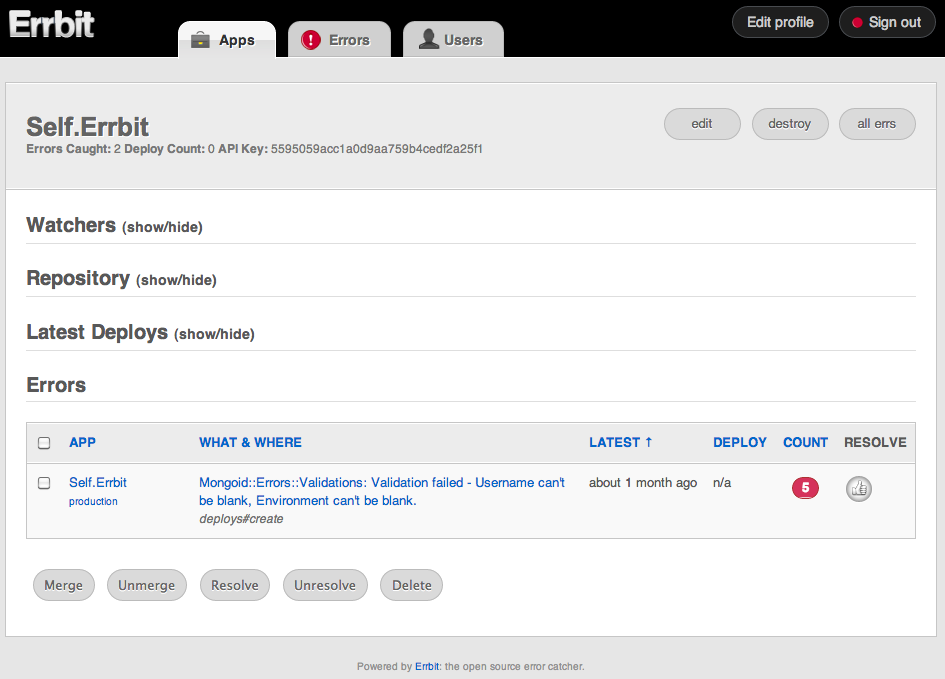
\includegraphics[width=10cm]{visualisation_des_erreurs.png}
  \end{overlayarea}
\end{frame}

\begin{frame}
  \begin{overlayarea}{10cm}{0.5cm}
    \centering
    \huge
    Information concernant une erreur
    \par
  \end{overlayarea}
  \begin{overlayarea}{10cm}{6cm}
    \centering
    \vfill
    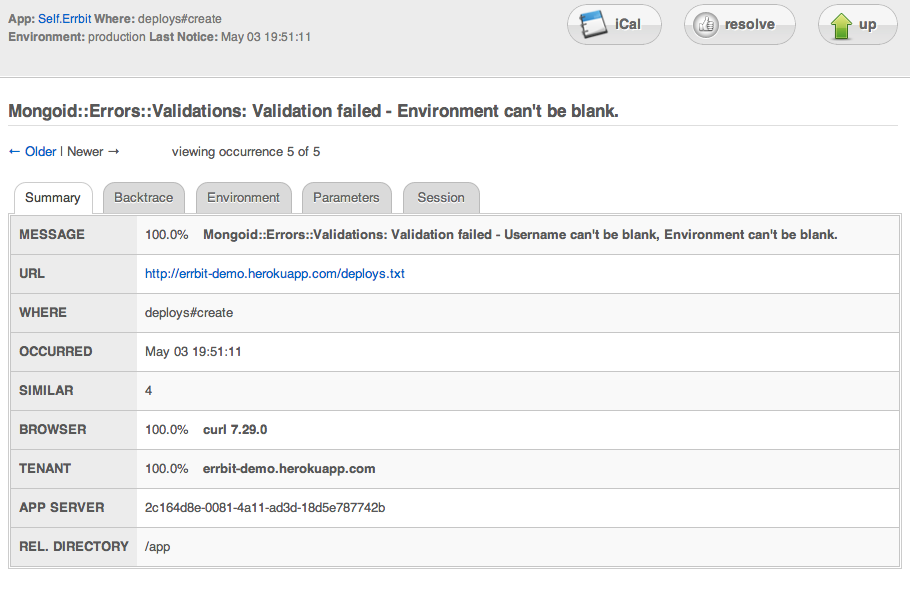
\includegraphics[width=\linewidth]{visualisation_d_une_erreur.png}
  \end{overlayarea}
\end{frame}

\begin{frame}
  \begin{overlayarea}{10cm}{0.5cm}
    \centering
    \huge
    Association à un Bug Tracker
    \par
  \end{overlayarea}
  \begin{overlayarea}{10cm}{3cm}
    \centering
    \vfill
    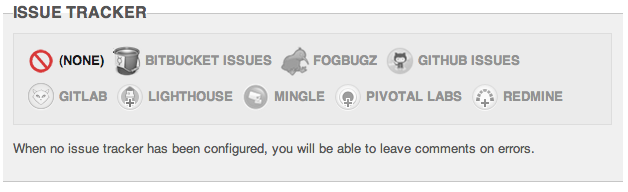
\includegraphics[width=\linewidth]{issue_tracker.png}
  \end{overlayarea}
\end{frame}

\begin{frame}
  \begin{overlayarea}{10cm}{0.5cm}
    \centering
    \huge
    Plusieurs systèmes de notifications
    \par
  \end{overlayarea}
  \begin{overlayarea}{10cm}{3cm}
    \centering
    \vfill
    
\includegraphics[width=\linewidth]{service_de_notification.png}
  \end{overlayarea}
\end{frame}


\end{document}
